\begin{table}[t]%[htpb]
\caption{Try-Catch Statement Detecting Comparison (Evaluate {\xstate} As Individual --- Block Level) (RQ2)}
  \vspace{-12pt}
  \small
	\begin{center}
		\renewcommand{\arraystretch}{1}
		\begin{tabular}{| p{3.05cm}<{\centering} | p{1.2cm}<{\centering} | p{1.2cm}<{\centering}| p{1.2cm}<{\centering}|}
		  \hline
			  & Precision  & Recall & F1-score \\
			\hline
			CodeBERT w/o fine-tuning &  0.0 & 0.0  & 0.0\\
			\hline
			{\xstate}  & \textbf{0.4}  &  \textbf{0.6369} & \textbf{0.4914}\\
			\hline
		\end{tabular}
		\label{tab:xstate-block}
	\end{center}
\end{table}

We also evaluate {\xstate} as individual at the try-catch block level (see Figure~\ref{tab:xstate-block}). The Codebert baseline still produce no correct prediction, while {\xstate} achieves 40\% of precision and about 63\% of recall. 

\begin{figure}[t]
 	\centering
 	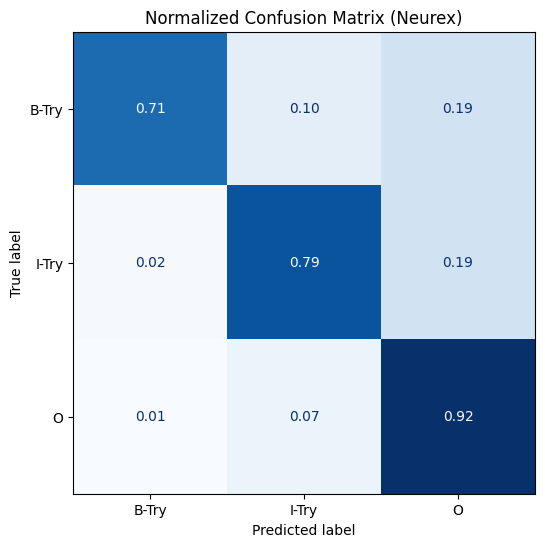
\includegraphics[width=2.4in]{rq2_cm_neurex.png}
        \vspace{-10pt}
 	\caption{Normalized Confusion Matrix --- {\tool} (XState Evaluated As Individual) (RQ2)}
 	\label{fig:rq2-cm-codebert}	
\end{figure}

\begin{figure}[t]
 	\centering
 	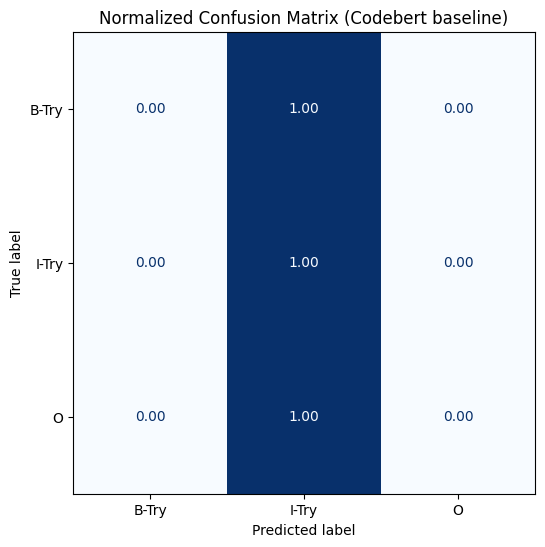
\includegraphics[width=2.4in]{rq2_cm_codebert.png}
        \vspace{-10pt}
 	\caption{Normalized Confusion Matrix --- CodeBERT baseline (XState Evaluated As Individual) (RQ2)}
 	\label{fig:rq2-cm-neurex}	
\end{figure}